\documentclass[10pt]{book}

\usepackage{cdtBook}
\usepackage{requerimientos}

\title{Sistema de Control Radiológico V2.0\\ Etapa I}
\subtitle{\bigskip Propuesta de desarrollo}

%\title{Propuesta Detallada}
%BESP
%\subtitle{Subsistema Banco de Imágenes\\Sistema de Información y Documentación Ambiental}
\author{Coordinación de Desarrollo Tecnológico}
%\organization{Escuela Superior de Cómputo, IPN}
%\date{15 de Junio de 2012}




\proyecto[SCOR]{Sistema de Control Radiológico V2.0}
\etapaProy{Inicial}
\usoProy{Externo}

\documento[D--PR]{Propuesta de Desarrollo}
\docVersion{1.0}
%\docFecha{}

%\docRefs{
%	\DRitem{Anexo Técnico}{Anexo Técnico del convenio de colaboración ESCOM-SMA.}
%}

\elaboro[Analista IPN]{José Jaime López Rabadán}
\superviso[Jefe de UPIS de ESCOM]{Ulises Vélez Saldaña}
\aprobo[Responsable del proyecto]{Fernando Ramirez Perez}

 
\begin{document}


\pagestyle{empty}
\ThisURCornerWallPaper{0.4}{images/logos.png}
\maketitle
%\makeDocInfo[9cm]
\frontmatter
\tableofcontents
\mainmatter
\pagestyle{fancy}

% \ThisURCornerWallPaper{0.5}{images/logos2.png}
% \maketitle
% \tableofcontents

%=========================================================
\chapter{Introducción} 

\section{Presentación}

	El presente documento contiene la Propuesta de Desarrollo para una nueva versión de {\bf Sistema de Control Radiológico}\footnote{Conocido por los usuarios como SCOR.} denominado SCOR 2.0 por parte de la Coordinación de Desarrollo Tecnológico de la Escuela Superior de Cómputo\footnote{De aquí en adelante se utilizan las siglas ESCOM para referirse a esta escuela.} del Instituto Politécnico Nacional\footnote{De aquí en adelante se utilizan las siglas IPN.}.
	
	La propuesta inicia con la presentación del resultado del análisis realizado y la descripción de los problemas detectados y las necesidades externadas por las áreas de la Comisión Nacional de Seguridad Nuclear y Salvaguardias\footnote{De aquí en adelante se utilizan las siglas CNSNS.} involucradas con el sistema.

\section{Antecedentes} 

\Instrucciones{Resumen del proyecto: nombre, partes involucradas, objetivo, alcance, sede, administración, gobierno, fechas de entrega, status actual}

	La presente propuesta es el resultado de un estudio realizado por analistas de la Coordinación de Desarrollo Tecnológico a petición de la Comisión Nacional de Seguridad Nuclear y Salvaguardias de la Secretaría de Energía.
	
	El objeto de dicho análisis es la revisión del proceso y sistemas existentes para  otorgar, renovar y revocar licencias para el manejo de Material Redioactivo, así como para llevar a cabo la inspección correspondiente a las instalaciones de los permisionarios de dichas licencias. 
	

\section{Confidencialidad}

	La presente propuesta se elaboró con base en entrevistas realizadas con la CNSNS y el personal del IPN asignado a este proyecto. La información contenida en este documento es una estimación inicial sujeta a negociación y está dirigida a las personas descritas al final de este documento. Se exige que la información contenida en esta propuesta no sea compartida a terceros, en especial a otros proveedores participantes en el concurso del proyecto en cuestión, sin la autorización previa del IPN mediante el contacto provisto al final del documento.


%=========================================================
\chapter{Diagnóstico} 

	Este capítulo presenta la problemática detectada y ofrece un conjunto de posibles alternativas de solución enfatizando la correspondiente a esta propuesta junto con sus ventajas y desventajas.
	
%---------------------------------------------------------
\section{Situación actual}

	Actualmente la CNSNS es la encargada de ofrecer el trámite para la obtención, supervisión, renovación y revocación de las licencias para el uso, transportación, adquisición y disposición final de material radioactivo.
	
\subsection{Proceso de Licenciameinto}

	La figura~\ref{fig:procesoLic} muestra el proceso para el licenciamiento a grandes rasgos. No es posible detallar cada proceso de manera simple debido a que existen diferentes vertientes del proceso en función del tipo y uso que se le dará a la fuente del material radioactivo. Sin mencionar a las diferentes áreas que están involucradas en el proceso. Cada actividad del proceso es un proceso en sí y se puede detallar en gran parte en función del tipo de licencia que se desea adquirir.

\begin{figure}[htbp!]
	\begin{center}
		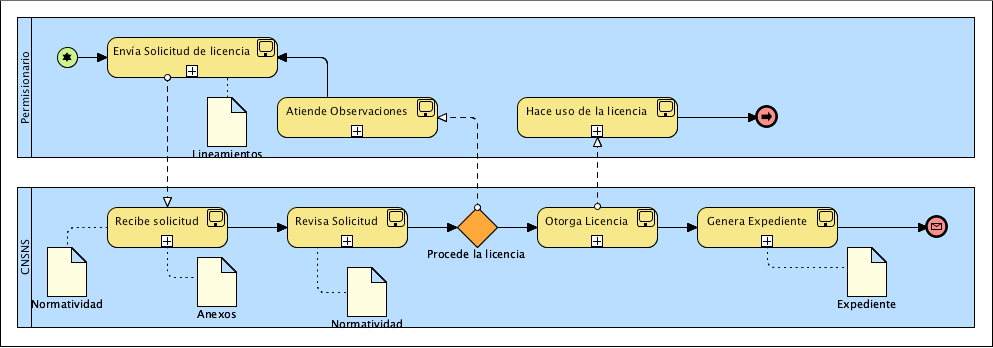
\includegraphics[width=\textwidth]{images/procesoLic}
		\caption{Proceso de licenciamiento.}
		\label{fig:procesoLic}
	\end{center}
\end{figure}

	Mucha de la información que determina el flujo y las reglas de operación para decidir si se otorga una licencia o no, depende del tipo de fuente radiológica, de los instrumentos que la ocupan y de las prácticas y usos que se le darán. Toda esa información se encuentra en los anexos mencionados en el proceso.
	
	Por otro lado el proceso para la renovación es muy parecido al del licenciamiento, solo que se puede simplificar y reducir la cantidad de información requerida ya que en principio es la misma que la de la licencia pasada. El trámite de modificación se parece mucho al de renovación, solo que se agrega la información en relación a los cambios, ampliación o reedición de las prácticas o usos de la fuente radiológica.
	
\subsection{Proceso de Inspección}

	La supervisión es un proceso diferente, ya que una vez otorgada una licencia existen momentos establecidos en que se debe o puede hacer una inspección en sitio a fin de corroborar el correcto uso y funcionamiento de las fuentes radioeléctricas.
	
	La figura~\ref{fig:procesoInsp} muestra el proceso en general. En esta parte del proceso es importante considerar que la inspección depende mucho de la información que se generó en el licenciamiento, ya que sobre eso va la inspección. El aspecto mas relevante a considerar es que si la fuente está siendo usada de manera irresponsable al grado de que la vida de las personas corre peligro, se puede cancelar la operación y se retiran las fuentes del lugar, quedando a resguardo de la CNSNS. 
	
\begin{figure}[htbp!]
	\begin{center}
		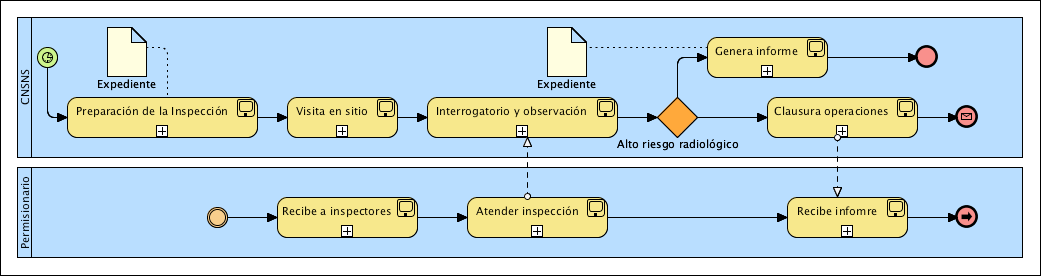
\includegraphics[width=.8\textwidth]{images/procesoInsp}
		\caption{Proceso de Inspección.}
		\label{fig:procesoInsp}
	\end{center}
\end{figure}


\subsection{Sistema SCOR}

	Actualmente existe un sistema llamado SCOR (Sistema de Control Radiológico) el cual se desarrolló con la finalidad de apoyar el licenciamiento y la inspección en materia de material radiológico.
	
	La figura~\ref{fig:scor} muestra la forma en que actualmente se utiliza SCOR. Este sistema se desarrolló como una aplicación de escritorio diseñada para un solo usuario. Al ser actualmente varios los usuarios que requieren utilizar el sistema, esta limitante se supera por medio del acceso al servidor en donde vive la aplicación mediante el acceso con Escritorios Remotos. La seguridad se controla mediante los permisos otorgados por Active Directory\footnote{El sistema de manejo de cuentas de usuarios que utiliza Windows Server. Tanto Active Directory como Widnows y Wosdiws Server, son marcas registradas de Microsoft Corporation.}.
	
	En cuanto a su funcionalidad, SCOR no está terminado y varios módulos, los relacionados con la Inspección no han sido terminados del todo, por lo que parte del trabajo se realiza en Excel y Word.
	
	La información relacionada con el licenciamiento se carga en este sistema, aunque mucha se registra previamente en otro sistema llamado BD1, del cual hablaremos a continuación.
	
	
\begin{figure}[htbp!]
	\begin{center}
		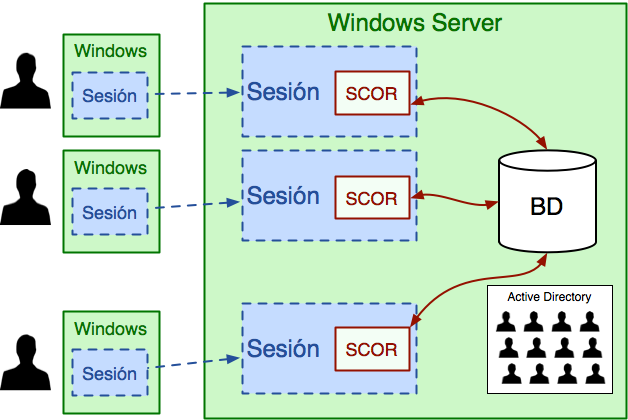
\includegraphics[width=.7\textwidth]{images/scor}
		\caption{Arquitectura del Sistema de Control Radiológico}
		\label{fig:scor}
	\end{center}
\end{figure}


\subsection{Sistema BD1}

	El sistema BD1 se ejecuta de una forma similar a la de SCOR, solo que esta corre bajo Access. Esta plataforma ejecuta tanto a la aplicación como a la BD en un solo archivo, haciendo que los bloqueos a tablas o registros sea imposible, ver figura~\ref{fig:bd1}.
	
\begin{figure}[htbp!]
	\begin{center}
		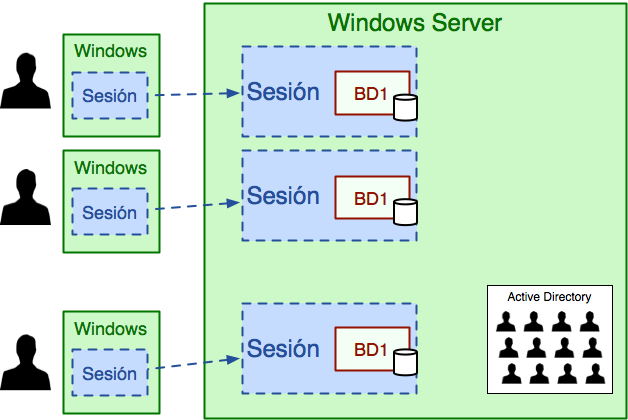
\includegraphics[width=.7\textwidth]{images/bd1}
		\caption{Arquitectura del sistema BD1.}
		\label{fig:bd1}
	\end{center}
\end{figure}
	

	Este sistema tiene mucha funcionalidad ademas de la relacionada con el licenciamiento, ya que registra todos los trámites, oficios y documentos que llegan a la CNSNS y su paso a través de todas las áreas.
	
	Es por esta razón que las diferentes áreas registran mucha información contenida en los documentos que se reciben, incluyendo aquella relacionada con los trámites de licenciamientos. Gran parte de la información contenida en este sistema suele estar incluso mas actualizada que la que aparece en SCOR.
	
	Durante el proceso de inspección, el personal encargado encuentra muy útil la información almacenada en este sistema. Sin embargo, en la mayoría de los casos se debe acceder al expediente físico almacenado en archivo para constatar toda la información.


%---------------------------------------------------------
\section{Problemas Detectados}
	
	Con base en la revisión de los procesos anteriores y sistemas existentes, se recopilaron las impresiones y comentarios de los actores del proceso. Los problemas detectados se resumen a continuación:
	
	\begin{itemize}
		\item Plataforma inadecuada. El uso de escritorios remotos genera que se ejecuten varios entornos gráficos y escritorios, saturando los servicios, memoria y transito en la red.
		\item Bajo desempeño. Ya que el servidor se tarda mucho tiempo ye contestar por el alto tráfico generado por los escritorios remotos.
		\item Información redundante. Mucha de la información requerida se encuentra en dos sistemas.
		\item Falta de Históricos. El sistema solo contempla el registro, por lo que cualquier actualización modifica la información capturada anteriormente, por lo que no es posible saber desde cuando se actualizó cada dato, ni que información tenia el sistema anteriormente.
		\item Poca confiabilidad. Se puede borrar información importante en el sistema  y hay otra que debería ser obligatoria y se puede omitir en la captura.
		\item Funcionalidad incompleta. El sistema SCOR está sin terminar.
		\item Duplicidad de trabajo. La información se debe capturar dos veces, generando retrasos en la operación.
		\item Funciones acopladas. Actualmente el sistema BD1 integra funcionalidad tanto de licenciamiento como de la Gestión interna de la CNSNS.
		\item Riesgo del Expediente físico. Ya que se solicita por diversas áreas para el licenciamiento y la inspección.
		\item Información desactualizada. Es difícil saber cual de los dos sistemas es el mas actualizado.
		\item Poca visibilidad del proceso. Es difícil saber el estado actual de cada trámite, ya que hay que meterse a BD1 y verificar banderas y tablas específicas para cada trámite.
		\item No hay información para la alta gerencia. Los directivos no tienen una vista del sistema que les permita conocer el estatus global de los trámites y tomar decisiones.
	\end{itemize}

%---------------------------------------------------------
\section{Identificación de Causas}

Derivado de la problemática anterior se realizó una estimación de las posibles acudas:

\begin{itemize}	
	\item Plataforma inadecuada. Aun cuando los escritorios remotos resuelven el problema, no fueron diseñados para utilizarse de esta forma.
	\item Crecimiento inesperado. El sistema BD1, al contener la información de todos los oficios que se reciben, ha sido enriquecido por diferentes áreas que solicitan agrega información que pueda ser relevante para su área.
	\item Falta de políticas adecuadas para el manejo de sistemas. El manejo de políticas, permitiría que se identifiquen necesidades específicas y agruparlas para generar estrategias adecuadas para el desarrollo tecnológico de la CNSNS.
	\item Redundancia del trabajo. La redundancia de responsabilidades genera trabajo repetitivo y duplicidad de información y desactualización.
	\item Sistema incompleto. La razón por la que se duplique la información o se acceda al expediente físico, s debe a que el SCOR no cuenta con las funciones requeridas.
	\item El Sistema actual no considera que se deben generar informes y tomar desicione spor parte de las direcciones de la CNSNS.
\end{itemize}

%---------------------------------------------------------
\section{Estimación de Consecuencias}

\begin{itemize}	
	\item Incumplimiento en los tiempos. La duplicidad de funciones, trabajo e información, hace que se requiera demasiado tiempo para alcanzar los objetivos.
	\item Falta de supervisión. No se puede determinar con precisión que instituciones deben ser inspeccionadas o si ya lo fueron.
	\item Falta de conocimiento del estado de las licencias. Aunque se tienen los trámites en papel, llegará el momento en que será imposible obtener los datos en los tiempos requeridos para la operación, dado que el sistema no notifica ni tiene forma de consultar esta información.
	\item Caos en la información. Con un alto volumen de información, se perderá el control de lo que se contiene en ambos sistemas.
	\item Desuso de los sistemas actuales. El SCOR empieza a dejar de ser utilizado por el personal.
\end{itemize}

%---------------------------------------------------------
\section{Otros aspectos}

	Se considera importante que la inspección se realice con una lista de verificación (checklist) y cuestionario abiertos ya que es muy variada la cantidad de preguntas o aspectos a considerar.
	
	Además se tiene planeada la apertura de una Ventanilla de atención que permita a los permisionarios agilizar el trámite y proporcionar su información vía Internet.
	
	Otro aspecto a considerar es que los sistemas deben alinearse e interoperar en lo posible con el VUCEM\footnote{Ventanilla Única de Comercio Exterior Mexicano, sistema mediante el cuan se implementa la Ventanilla Digital Mexicana de Comercio Exterior} ya que existe información que debe fluir desde y hacia este sistema.
	
	Además, se solicita considerar un mecanismo confiable de autenticación ({\em uso de una firma electrónica}) para que los solicitantes y permisionarios puedan realizar sus trámites de manera electrónica.

%---------------------------------------------------------
\section{Conclusión del análisis}

	La CNSNS debe establecer de manera consistente los flujos, responsabilidades y alcances de las actividades de cada área involucrada en los procesos de licenciamiento e inspección a fin de que los sistemas involucrados puedan operar adecuadamente.
	
	El sistema BD1 es un sistema rebasado en sus atribuciones originales y que incorpora actualmente funciones de diferentes áreas y que de seguir creciendo, terminará por dejar de ser útil para todas las áreas.
	
	Una de las principales necesidades actualmente es el aislamiento del sistema de Gestión interna (BD1) y las necesidades de las demás áreas.
	
	El sistema SCOR V2.0 debe contemplar la gerencia, toma de decisiones e inspección de los permisionarios así como su uso en las ventanillas mencionadas en la sección anterior.
	
	Con base en lo anterior se considera que el desarrollo pueda llevar un proceso con las siguiente setapas:
	
\begin{itemize}
	\item Análisis y definición de los procesos de licenciamiento e inspección.
	\item Diseño del mecanismo de interacción con el VUCEM.
	\item Determinación del mecanismo de autenticación para solicitantes y permisionarios.
	\item Rediseño e implementación de los sistemas SCOR y de Gestión Interna (Actualmente BD1).
	\item Apertura de la Ventanilla para Licencias.
	\item Integración con el VUCEM.
	\item Migración de información.
	\item Implementación del nuevo proceso y puesta en marcha de los nuevos sistemas.
\end{itemize}

%=========================================================
\chapter{Alcance de la Propuesta}

	La siguiente propuesta plantea la primera etapa del proyecto considerando cinco meses como tiempo disponible.

%---------------------------------------------------------
\section{Objetivo General}

	Elaboración de análisis de requerimientos y prototipo conceptual del SCOR Versión 2.0 considerando la Ventanilla para solicitud de licenciamiento y el diseño de la Interoperabilidad con el VUCEM.

%---------------------------------------------------------
\section{Objetivos Específicos}

\begin{itemize}
	\item Análisis de los procesos de licenciamiento e inspección.
	\item Elaboración del prototipo conceptual.
	\item Análisis técnico del VUCEM.
	\item Diseño de la estrategia de interoperabilidad con el VUCEM.
\end{itemize}

%---------------------------------------------------------
%\section{Requerimientos}
%
%
%\subsection{Modelo de Despliegue}
%
%\subsubsection{Hardware}
%
%\subsubsection{Software}

%\subsection{Requerimientos funcionales}
	
	
%=========================================================
\chapter{Metodología}


%---------------------------------------------------------
\section{Proceso}

	La elaboración del análisis y construcción del prototipo conceptual se llevará mediante el siguiente proceso:
	
	
\begin{enumerate}
	\item {\bf Toma de Requerimientos.} Mediante mesas de trabajo, entrevistas personales, elaboración de encuestas, inspección de la operación y análisis documental de evidencias, normas y reglamentos aplicables se integra el expediente base para la realización del análisis.
	\item {\bf Organización y análisis.} Se aplica un proceso de organización y análisis de la problemática que permitirá determinar: el nuevo proceso a seguir y la funcionalidad que deberá presentar el sistema. Esto con base en un enfoque de aprovechamiento de las distintas áreas de oportunidad identificadas y la aplicación de nuevas tecnologías de información en la operación.
	\item {\bf Verificación y retroalimentación del diseño.} Mediante mesas de trabajo, entrevistas y retroalimentación con la CNSNS se presentan los resultados del análisis a fin de verificar la viabilidad y alcance de su aplicación con base en los recursos y capacidades del personal, tecnología e infraestructura de la CNSNS.
	\item {\bf Especificación formal del sistema.} Se genera un documento detallado y conciso con todos los detalles que deberá tener el nuevo proceso y el SCOR V2.0 para su aprobación.  
	\item {\bf Aprobación de acuerdos.} Una vez establecidos los acuerdos, se presenta la especificación para su lectura, análisis y aprobación por ambas partes.
	\item {\bf Presentación del Prototipo Conceptual.} Se construye y presenta una maqueta del sistema ({\em Prototipo Conceptual}) que permita evaluar la interacción del sistema con los usuarios.
\end{enumerate}

%---------------------------------------------------------
\section{Especificación Formal}

	Consiste en un documento que contiene la siguiente información:
	
\begin{itemize}
	\item {\bf Introducción.} Contiene la presentación del documento, contenido, organización, etc.
	\item {\bf Modelo del negocio.} Presenta las consideraciones propias de la operación y la organización que gobiernan al sistema, entre ellas: Glosario de términos, normatividad aplicable, procesos, roles, modelo estructural del negocio y reglas de operación.
	\item {\bf Modelo de despliegue.} Especifica las características de Software, Hardware y servicios de comunicación necesarios para que opere el sistema y la arquitectura del sistema.
	\item {\bf Modelo del Comportamiento.} Describe mediante casos de uso toda la funcionalidad paso a paso del sistema especificando, el propósito de cada funcionalidad del sistema, las operaciones involucradas, los efectos colaterales de cada operación, los prerequicitos, el control de acceso a las operaciones y las responsabilidades, tanto de los usuarios como del sistema, durante la operación.
	\item {\bf Modelo de interacción.} Especifica, a manera de manual de usuario todas las interfaces del sistema y la forma en que deben usarse, incluyendo una lista con todos los mensajes, correos, avisos y notificaciones que pueda generar el sistema.
\end{itemize}


%---------------------------------------------------------
\section{Ambiente de Pruebas}

	El ambiente de pruebas consiste en una carpeta con archivos en formato HTML, que contiene el Prototipo Conceptual y se puede utilizar para verificar el comportamiento que tendrá el sistema.

%---------------------------------------------------------
\section{Entregables}
	
	Al término del proyecto los productos que se entregarán son:
	
\begin{description}
	\item [Entregable I.] Expediente de análisis. Carpeta con toda la documentación recabada, informes y evidencias de las entrevistas y mesas de trabajo
	\item [Entregable II.] Diagnóstico inicial. Contiene el análisis de la problemática, las oportunidades de mejora de procesos y las tecnologías que se pueden aprovechar en la operación.
	\item [Entregable III.] Especificación Formal. Que contiene la especificación del SCOR V2.0.
	\item [Entregable IV.] Prototipo Conceptual. Construcción y programación de la navegación y mensajes de las pantallas del SCOR V2.0.
\end{description}


\section{Tiempos y Costos del proyecto}

	En esta sección se describen los tiempos y los montos correspondientes a cada entrega del sistema. Los  tiempos se consideran a partir de la firma del convenio.\\

\begin{tabular}{|l | l | r|}
	\hline
	{\bf Entregable}& {\bf Fecha} &{\bf Monto}  \\
	\hline
	I & Primeras dos semanas  & \$ 500,000.00+IVA\\
	\hline
	II & Mes y medio & \$ 700,000.00+IVA\\
	\hline
	III & Tercer mes & \$ 700,000.00+IVA\\
	\hline
	IV & Quinto mes & \$ 600,000.00+IVA\\
	\hline
	\hline
	 & Total & \$ 2,500,000.00+IVA\\
	\hline
\end{tabular}

\clossing

\end{document}